\documentclass[a4paper]{article}

\usepackage{numprint}
\usepackage{nameref}
\usepackage{float}
\usepackage{url}
\usepackage{graphicx}	% For figure environment
\usepackage{epstopdf}
\usepackage[center]{subfigure}
\usepackage{amssymb}	% For mathematical figures like \mathbb{R}
\usepackage{amsmath}
\usepackage{framed}
\usepackage{tikz}
\usetikzlibrary{mindmap,trees}
\usepackage{pdflscape}
\usepackage[a4paper]{geometry}
\usepackage{subfiles}
\usepackage{listings}

\definecolor{dkgreen}{rgb}{0,0.6,0}
\definecolor{gray}{rgb}{0.5,0.5,0.5}
\usepackage{array}
\usepackage{booktabs}% http://ctan.org/pkg/booktabs
\usepackage{xparse}% http://ctan.org/pkg/xparse
% Rotation: \rot[<angle>][<width>]{<stuff>}
\NewDocumentCommand{\rot}{O{45} O{1em} m}{\makebox[#2][l]{\rotatebox{#1}{#3}}}%
\definecolor{mauve}{rgb}{0.58,0,0.82}

\lstset{frame=tb,
  language=Java,
  aboveskip=3mm,
  belowskip=3mm,
  showstringspaces=false,
  columns=flexible,
  basicstyle={\small\ttfamily},
  numbers=none,
  numberstyle=\tiny\color{gray},
  keywordstyle=\color{blue},
  commentstyle=\color{dkgreen},
  stringstyle=\color{mauve},
  breaklines=true,
  breakatwhitespace=true
  tabsize=3
}


\title{Advanced Systems Lab - Milestone II} 
\author{Matthias Ganz (ganzm@ethz.ch)} 
\date{\today} 


\begin{document}

\maketitle

\pagebreak

\tableofcontents

\pagebreak

\begin{abstract}

This document describes an analytical model of the message queuing system which was build during Milestone I. Analytical studies are presented and compared with the results obtained before. Different behaviour between the model and observed values are explained.


\end{abstract}

\pagebreak

%% ----------------------------------------------
% Section - The System
%% ----------------------------------------------
\section{The System}

This chapter should briefly show the most important components of the System Under Test (SUT). The curious reader is referred to the document Milestone I \cite{milestone1}. In depth information about the technical details are stated there.


% ------------------------------------------------
% Figure 

\begin{figure}[H]
	\begin{center}
    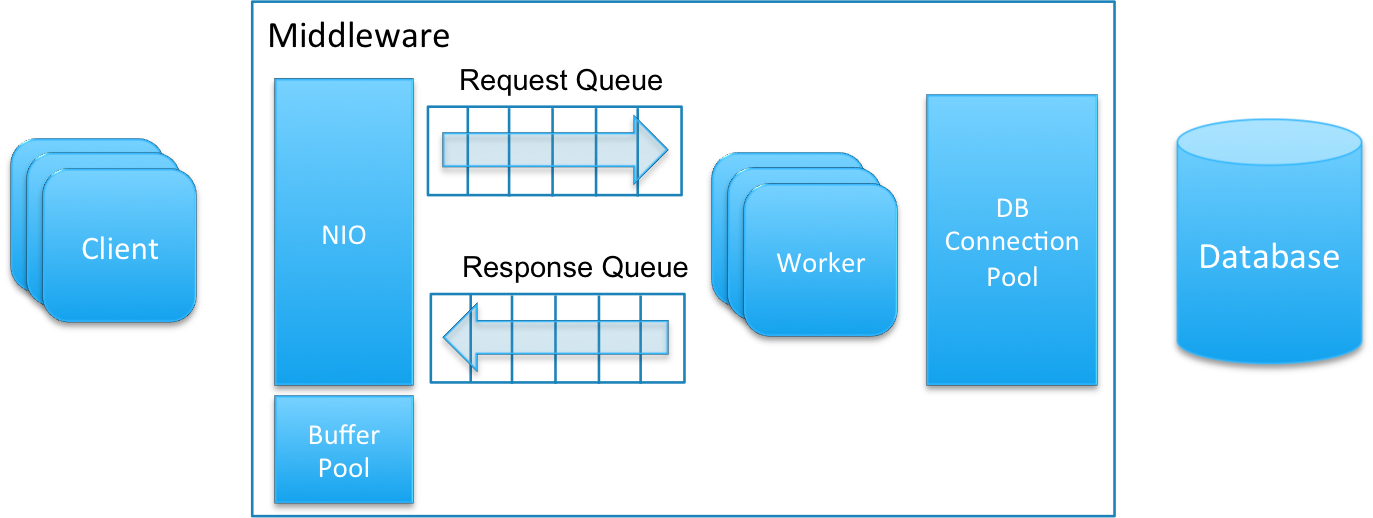
\includegraphics[scale=0.6]{../drawings/broker-threading.png}
  \end{center}
  \caption{System Under Test}
  \label{fig:sut}
\end{figure}

%% ----------------------------------------------

Requests from clients are read and pushed to Request Queue. This Queue is processed by a fixed numer of worker threads which utilize pooled database connections to generate an appropriate response. Theses responses are put back into the response queue which is processed by the networking interface.


%% ----------------------------------------------
% Section System Model
%% ----------------------------------------------
\section{Model of the System}
\label{sec:SystemModel}

\subsection{Modelling a closed system}
Due to the nature of the tests performed during Milestone I the system should be modeled as a closed queuing system. Each experiment was performed with a fixed number of clients. Each client is issuing at max one concurrent request. As long as the system is in its healthy boundaries no messages are discarded by the middleware. Therefore the number of messages in the system never exceed the number of clients.


% ------------------------------------------------
% Figure 

\begin{figure}[H]
	\begin{center}
    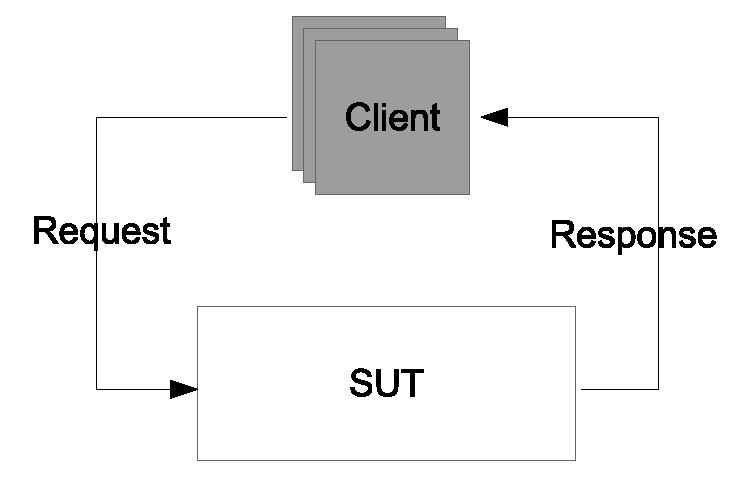
\includegraphics[scale=0.4]{../drawings-ms2/sut.eps}
  \end{center}
  \caption{Closed System}
  \label{fig:closedsystem}
\end{figure}

%% ----------------------------------------------



\subsection{Kendall's Notation}
In this chapter we look at the system as a black box and describe it with \textit{Kendall's Notation}. The 6 characteristic parameters A/S/m/B/K/SD are defined as followed.

\subsubsection{(A) Arrival Process}
\label{subsub:ArrivalProcess}

The interarrivaltime is modeled to be exponentially distributed. This can be shown from figure \ref{fig:interarrivaltime}. Data for this plot where obtained from a shortened 2 hour test with mixed types of clients. Therefore interarrivaltime is assumed to be \textit{Markovian (M)}.


% ------------------------------------------------
% Figure 

\begin{figure}[H]
	\begin{center}
    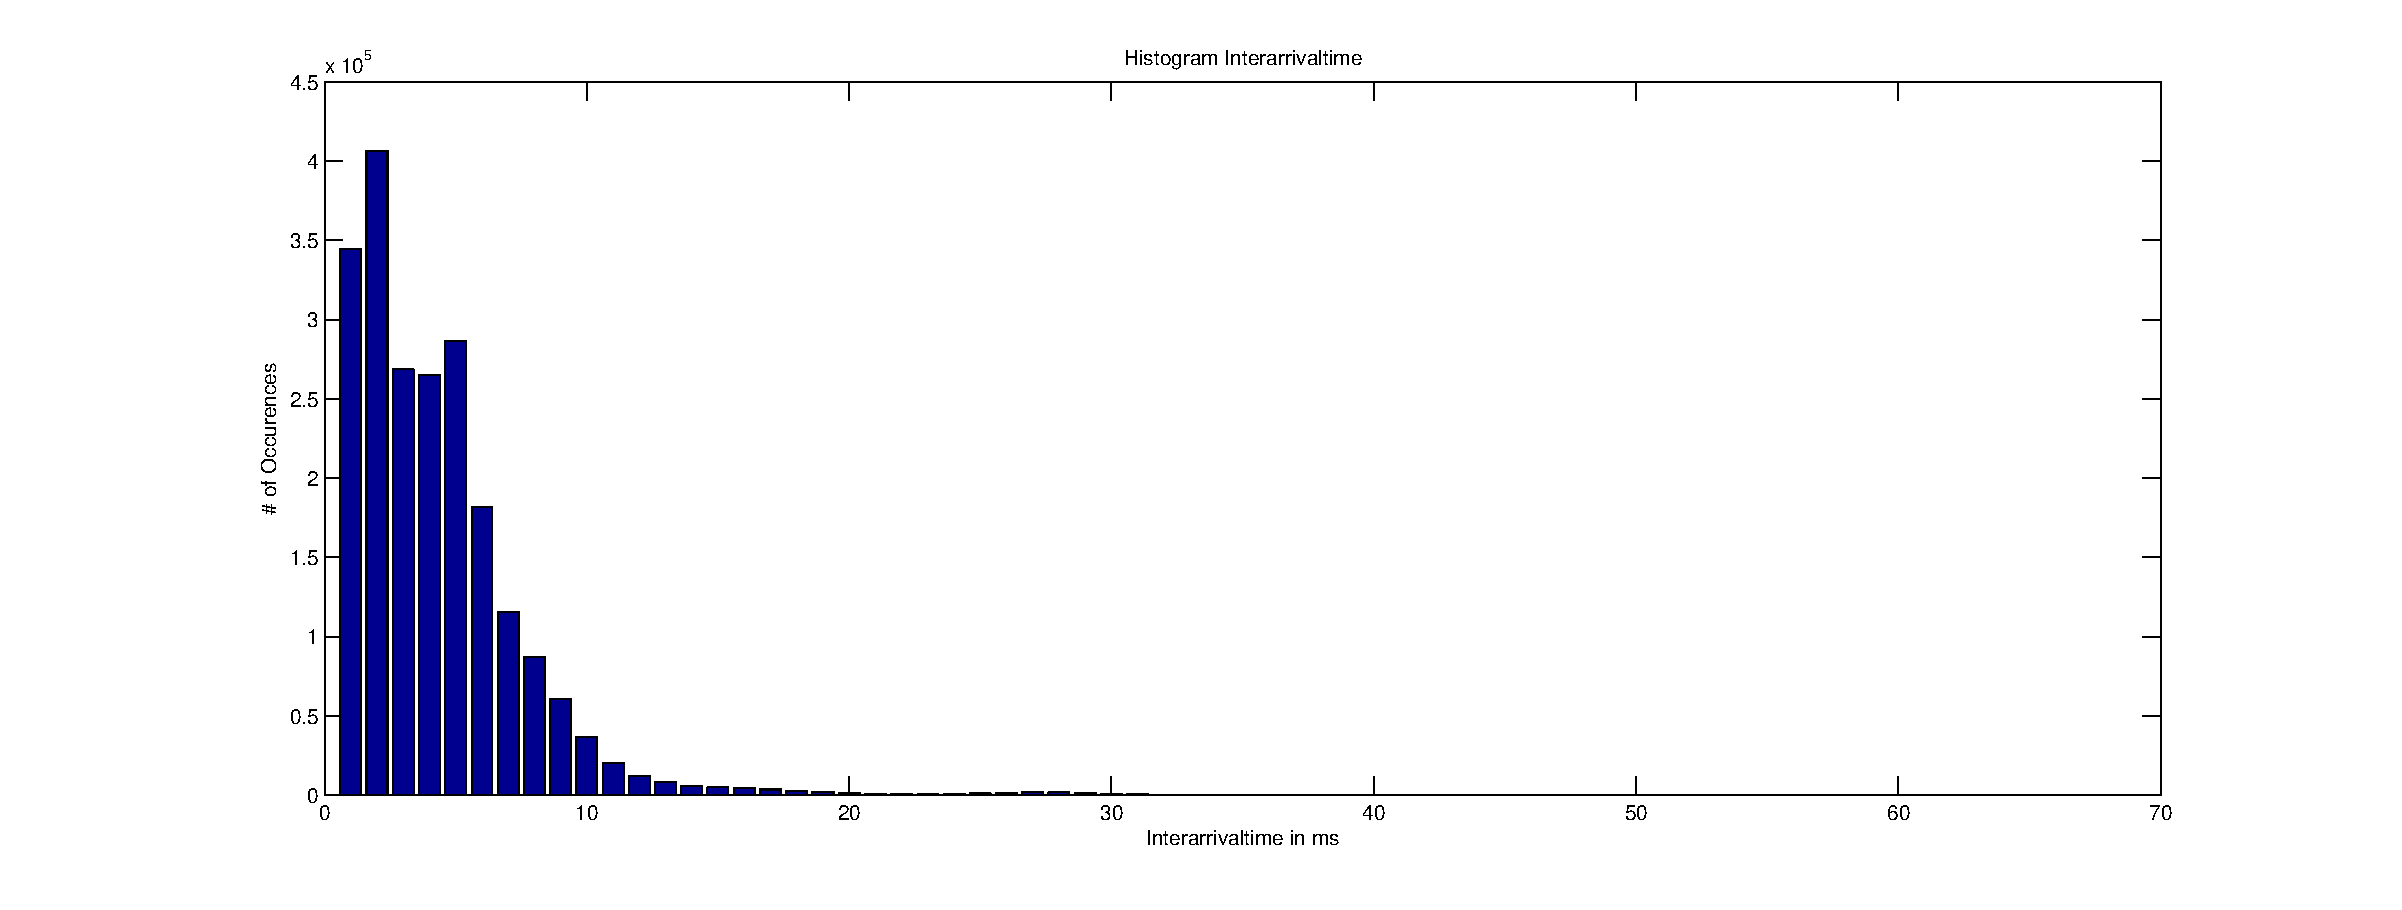
\includegraphics[scale=0.6]{../plots-ms2-mg/interarrivaltime.eps}
  \end{center}
  \caption{Histogram showing Interarrivaltime}
  \label{fig:interarrivaltime}
\end{figure}

%% ----------------------------------------------


\subsubsection{(S) Service Time Distribution }

Again it is assumed that the service time distribution is memoryless exponentially distributed. Data drawn from the same test as in chapter \ref{subsub:ArrivalProcess} show an exponential distribution of service time. Both blots do look quite similar.

% ------------------------------------------------
% Figure 

\begin{figure}[H]
	\begin{center}
    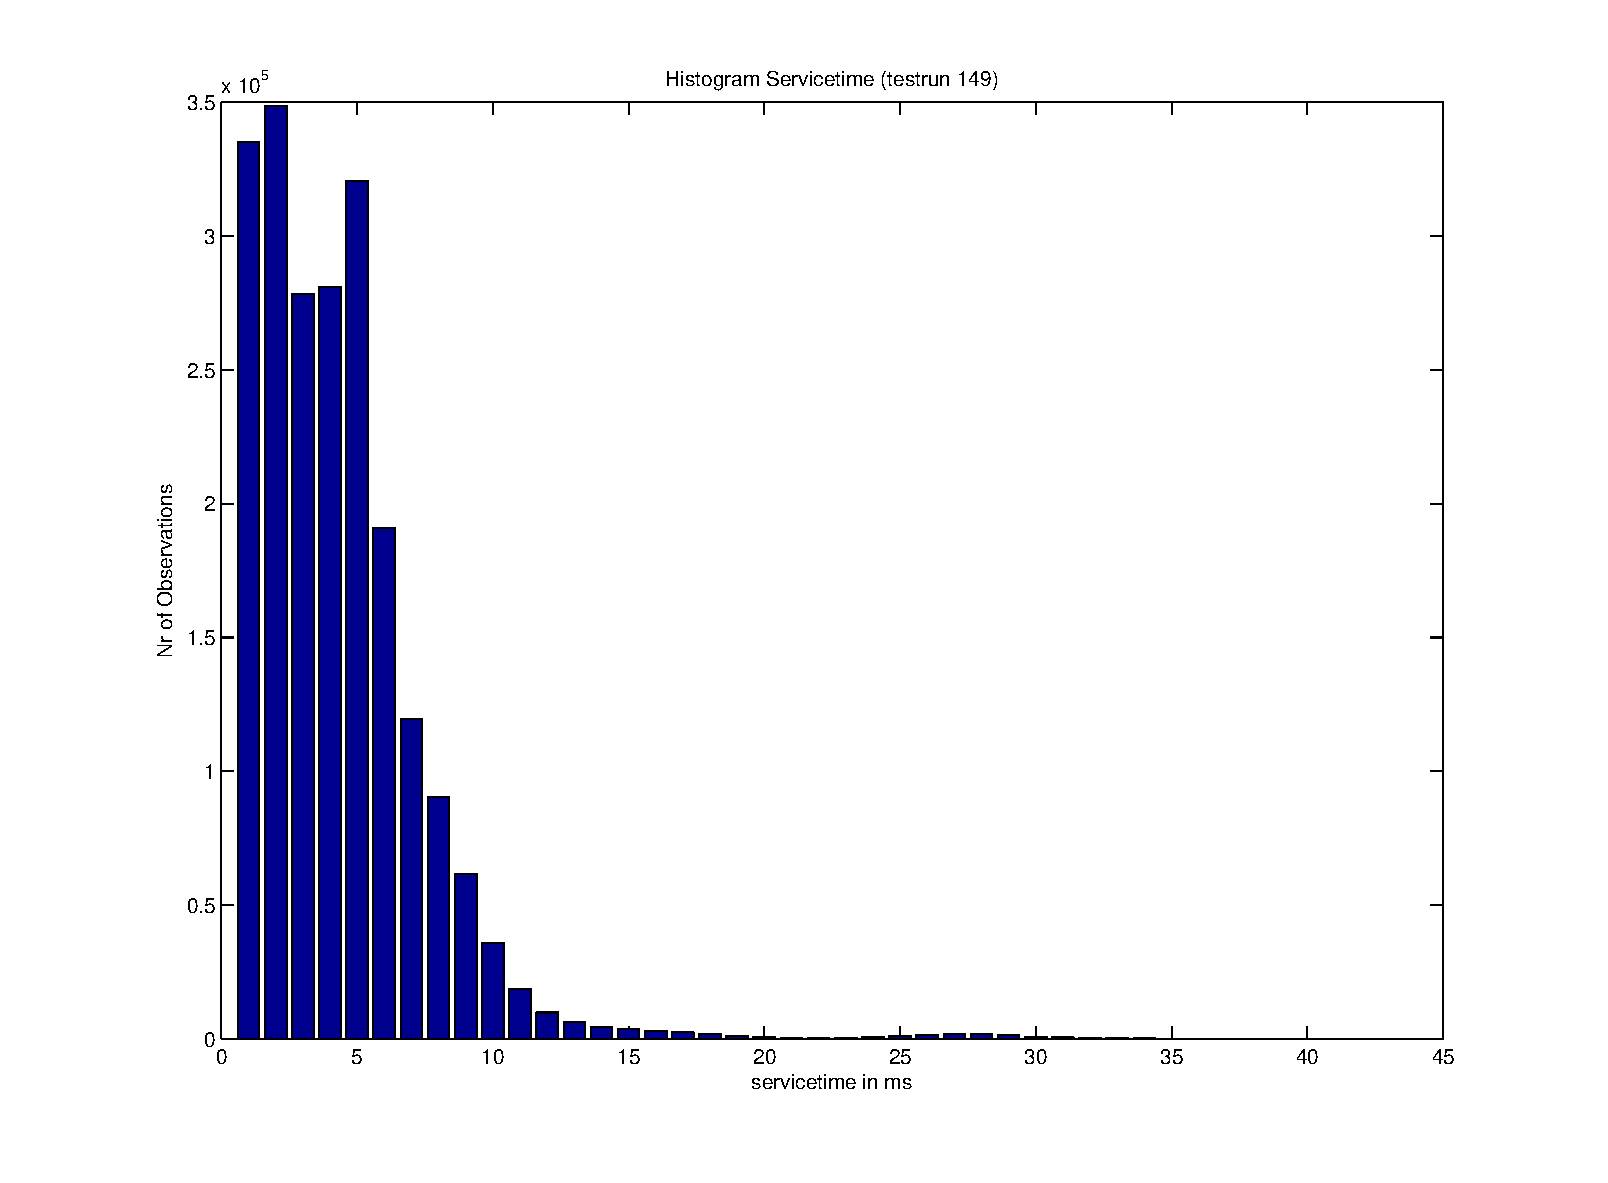
\includegraphics[scale=0.6]{../plots-ms2-mg/servicetime.eps}
  \end{center}
  \caption{Histogram showing Servicetime}
  \label{fig:servicetime}
\end{figure}

%% ----------------------------------------------


\subsubsection{(m) Number of Servers}

This parameter is determine by the number of middleware instances running.

\subsubsection{(B) Buffer - System Capacity }
In a first step the system capacity is assumed to be infinite.

\subsubsection{(K) Population Size}

Since we are modelling a closed system the population size can be set to the number of clients participating in the experiment.

\subsubsection{(SD) Service Discipline}
Because the whole messaging system consists of queues  First Come First Server (FCFS) service discipline is assumed for our system model.

\section{Refined System Model}
\label{sec:RefinedSystemModel}

Modelling the system as a black box is not very accurate. To be able to do a more distinct analysis and to identify bottle neck components the black box queue is refined into a queueing network.

Figure \ref{fig:systemmodel-singlebroker} shows the model of the system with only one middleware instance. It is modelled having four different service centers which are described in the following subsection.

% ------------------------------------------------
% Figure 

\begin{figure}[H]
	\begin{center}
    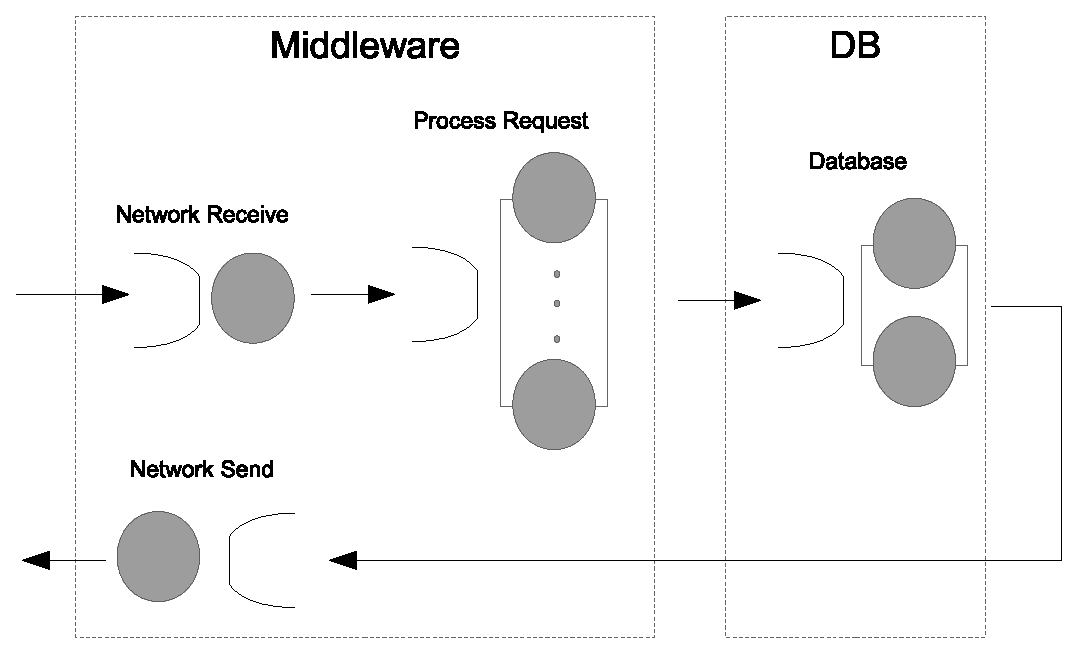
\includegraphics[scale=0.6]{../drawings-ms2/systemmodel-singlebroker.eps}
  \end{center}
  \caption{System Model with one Middleware}
  \label{fig:systemmodel-singlebroker}
\end{figure}

%% ----------------------------------------------

\subsection{Service Centers}

\subsubsection{Client}
The clients are modelled as Delay Centers. The time a client is sleeping between two requests is the think time $Z$.

\subsubsection{Network Receive}
\label{subsub:ServiceCenterNetworkReceive}

This service center represents the networking part where the middleware gets a request and buffers it until completely received. For this queue also the time used sending the request over the network is taken into account. The number of service nodes is 1 because receiving and buffering is done single threaded by the nio networking interface.\\

\begin{tabular}{|l|l|}
\hline 
Type & fixed capacity \\ 
\hline 
Queue Size & unbound\\ 
\hline 
Service Node Count & 1 \\ 
\hline 
\end{tabular} 

\subsubsection{Process Request}
This service center represents the request queue and the worker threads attached to it. The queue is represented by an actual queue and workers implemented in java. The queue size is fixed and corresponds with the size of the java queue (which is configurable and by default set to 100) \\

\begin{tabular}{|l|l|}
\hline 
Type & load dependent \\ 
\hline 
Queue Size & Corresponds to Request Queue size (default 100)\\ 
\hline 
Service Node Count & Corresponds to \# of worker thread \\ 
\hline 
\end{tabular} 

\subsubsection{Database}
This node represents the database. For the experiment an Amazon medium instance with two ECU's (EC2 Compute Units\footnote{Assumed to something equivalent to a CPU. Actually Amazon does not further explain the term ECU.}). However in a first attempt the service node count was set to 2. This however turned out to be not quite accurate (see section \ref{sub:QueueDatabase} for further explanations).  The queue size is modelled to be infinite because no refused database requests or timed out connections were observed during the experiment phase during milestone I. \\

\begin{tabular}{|l|l|}
\hline 
Type & fixed-capacity service center \\ 
\hline 
Queue Size & unbound \\ 
\hline 
Service Node Count & 12 \\ 
\hline 
\end{tabular} 


\subsubsection{Network Send}
This service center represents the networking part where the middleware sends back a response. Responses to transmit are buffered in a java response queue. So the queue size corresponds to the size of the java queue. As in section  \ref{subsub:ServiceCenterNetworkReceive} the service node count is one. \\

\begin{tabular}{|l|l|}
\hline 
Type & load dependent \\ 
\hline 
Queue Size & Corresponds to Response Queue size (default 100)\\ 
\hline 
Service Node Count & 1 \\ 
\hline 
\end{tabular} 

\subsection{Modelling Multiple Middlewares}
Taking into account more than one middleware instance would lead to the following model seen in figure \ref{fig:systemmodel-multiplebroker}.


% ------------------------------------------------
% Figure 

\begin{figure}[H]
	\begin{center}
    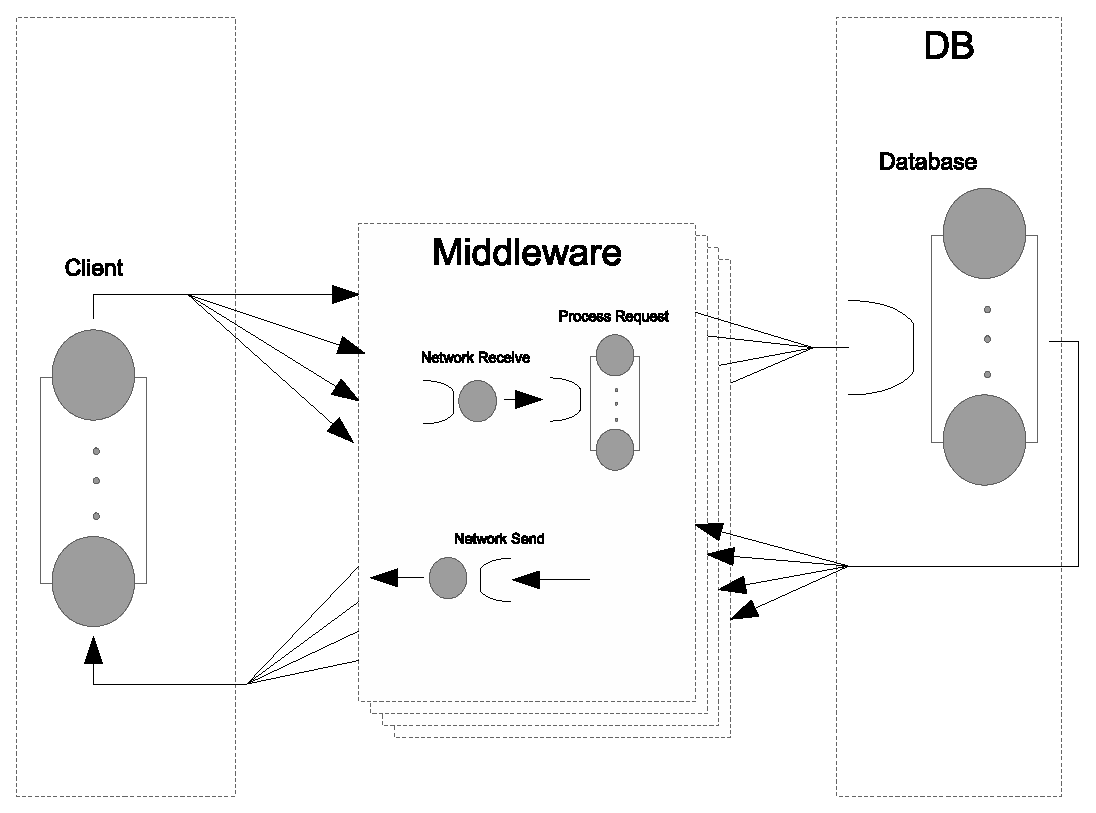
\includegraphics[scale=0.6]{../drawings-ms2/systemmodel-multiplebroker.eps}
  \end{center}
  \caption{System Model with multiple Middleware components}
  \label{fig:systemmodel-multiplebroker}
\end{figure}

%% ----------------------------------------------

Since clients and load is evenly distributed among multiple stateless middleware instances and the visit ratio $V_i$ of the $i$-th queue for $n$ instances is $1 \over n$. We can simplify the model by merging all of them together. This means that for each broker added the queue size and service node count is increased accordingly. However merging all middleware instances together leads us back to the model shown in figure \ref{fig:systemmodel-singlebroker} but with modified parameters.

\paragraph{For example} if there are 8 middleware the queue size of the \textit{Network Receive} component is still unbound but the service node count is 8 instead of 1 (it becomes a load dependent service center).


%% ----------------------------------------------
% Section Single Queues
%% ----------------------------------------------
\section{Analysing the Queues}

To further analyse the queues the experiment described in section \ref{sec:experiment} with a client count of 90 was taken. The system is nearly at maximum load but not yet saturated. All measurement values used in this chapter are taken from there. All the queues which have been modelled in the previous chapter are now instantiate with specific parameters.\\

To calculate the values which are presented in this and the further chapters a Java program was written which helps calculating characteristic number for the modelled queues.

\subsection{Network Receive - M/M/8}
\label{sub:QueueNwReceive}

Since we scale the number of middleware instances to 8 this queue becomes a M/M/8 queue. The queue size is still infinite. The arrival rate is the total number of requests divided by the experiment run time. The value for the mean service rate is is taken from the measurement from Milestone I. For that we take into account the network delay and the time taken by the middleware reading the network socket and putting the data into the Request Queue.\\

From the experiment the following values were measured:

\begin{tabular}{|c|l|l|}
\hline 
% arrival rate 47023 msg/30s / 8 broker
$\lambda$ & mean arrival rate & 195 requests / s \\ 
\hline 
$\mu$ & mean service rate & ${1 / {3ms}}$\\ 
\hline 
$m$ & number of service nodes & 8 \\ 
\hline 
\end{tabular} 

\subsubsection{Calculated Values}
\begin{equation}
\label{eq:TrafficIntensity}
\rho = \lambda / (m \mu)
\end{equation}


The following values were obtained by using the formulas from the book \cite[Box 31.2]{Raj}.\\

\begin{figure}[H]
\begin{center}
\nprounddigits{2}
\begin{tabular}{|l|r|}
\hline 
Traffic Intensity ($\rho$)& \numprint{0.562500000000000000000000000000000000000000000000000000000000000000000000000000000000000000000000000000000000000000000000000000000000000000000000000001}\\
\hline
Probability of Queueing & \numprint{0.004996678253810118287754045200141901428395110707714987388618561756962298075099102852842837348515043338671570100178407263991769762473888999513201437997}\\
\hline
Mean \# of Jobs in the System & \numprint{4.501229651289023583797376972060972421054644109275726735177667849182377440541918919842691792003736123946626206704340779912622974589983808620973951916390073594165218273735214030744349982262321450611161535626576422679780379712740612612143394645331435619582666053737477699092001028779690763875060849820250370003321746189881712245954799858098571604889292285012611381438243037701924900897147157162651484956661328429899821592736008230237526111000486798562003}\\
\hline
Mean \# of Jobs in the Queue & \numprint{0.001229651289023583797376972060972421054644109275726735177667849182377440541918919842691792003736123946626206704340779912622974589983808620973951916382073594165218273735214030744349982262321450611161535626576422679780379712740612612143394645331435619582666053737477699092001028779690763875060849820250370003321746189881712245954799858098571604889292285012611381438243037701924900897147157162651484956661328429899821592736008230237526111000486798562003}\\
\hline 
\end{tabular} 

\npnoround
\end{center}
\caption{Characteristic values for 'Network Receive'}
\label{tbl:queueanalysis-result-nwreceive}
\end{figure}


% ------------------------------------------------
% Figure 

\begin{figure}[H]
	\begin{center}
    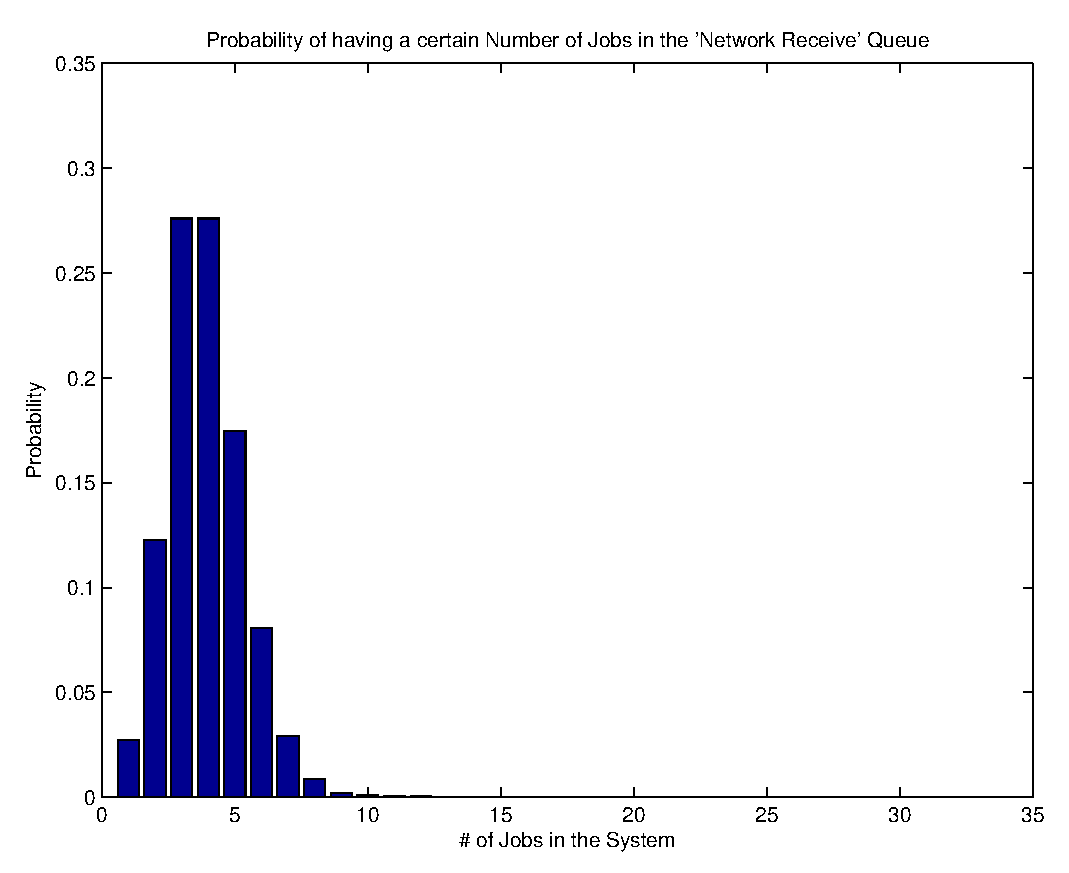
\includegraphics[scale=0.6]{../plots-ms2-mg/queueanalysis-1NwReceive.eps}
  \end{center}
  \caption{Probability of having a certain Number of Jobs in the 'Network Receive' Queue}
  \label{fig:queueanalysis1}
\end{figure}

%% ----------------------------------------------

\subsubsection{Explanation}

As seen from the calculated traffic  intensity this queue is not working nearly at capacity. There is almost no queueing at any time. Queueing happens only if there are more than 8 jobs in the system.

\subsection{Process Request - M/M/160/800}
This queue takes into account message deserialisation, processing and serialsation of the response. The number of service node corresponds to the total number of worker threads (20) times the number of middleware instances (8). Queue size matches the default queue size of 100 for each of the brokers. The arrival rate is the same as for the previous queue since no messages are lost.\\

\begin{tabular}{|c|l|l|}
\hline 
% arrival rate 47023 msg/30s
$\lambda$ & mean arrival rate & 195 requests / s \\ 
\hline 
$\mu$ & mean service rate & $1/1ms$ \\ 
\hline 
$m$ & number of service nodes & 160 \\ 
\hline 
\end{tabular} 

\subsubsection{Calculated Values}

% ------------------------------------------------
% Figure 

\begin{figure}[H]
	\begin{center}
    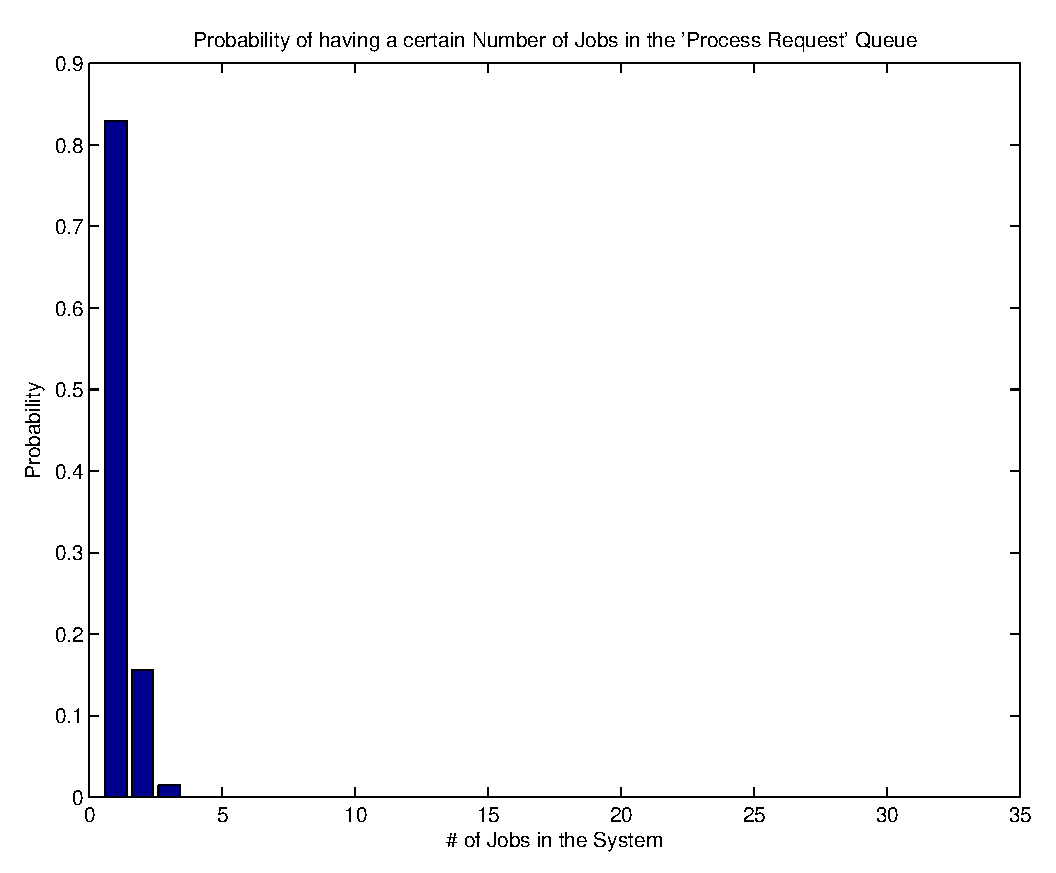
\includegraphics[scale=0.6]{../plots-ms2-mg/queueanalysis-2ProcessRequest.eps}
  \end{center}
  \caption{Probability of having a certain Number of Jobs in the 'Process Request' Queue}
  \label{fig:queueanalysis2}
\end{figure}

%% ----------------------------------------------


\begin{figure}[H]
\begin{center}
\nprounddigits{2}
\begin{tabular}{|l|l|}
\hline 
Traffic Intensity ($\rho$)& \numprint{0.009375000000000000000000000000000000000000000000000000000000000000000000000000000000000000000000000000000000000000000000000000000000000000000000000000}\\
\hline 
Probability of Queueing & \numprint{0}\\
\hline 
Mean \# of Jobs in the System & \numprint{1.285665595380242339401395452400300768646652659670658271275311493447245608470943401822097144423619853821366025757014136766249178203693466191165032240124}\\
\hline 
Mean \# of Jobs in the Queue & \numprint{0}\\
\hline 
\end{tabular} 
\npnoround
\end{center}
\caption{Characteristic values for 'Process Request'}
\label{tbl:queueanalysis-result-processrequest}
\end{figure}


\subsubsection{Explanation}

The calculated values are similar to the queue described in \ref{sub:QueueNwReceive}. The Traffic intensity is very low and the probability of queueing is almost 0. This indicates that for this experiment the number of worker threads is way too high and could be lowered significantly without loosing performance.


\subsection{Database - M/M/12}
\label{sub:QueueDatabase}

For the database the mean arrival rate of requests is 8 times higher than for the other queues. This is because the load is evenly spread accross all 8 middleware instances while there is only one database.

The number for the mean service rate was taken from the micro benchmark out of Milestone I. While evaluating the traffic intensity for this queue I recognized that setting the number of processing nodes to 2 as initially intended leads to a traffic intensity which is not stable any more ($>1$). I chose to estimate number of service nodes as following. As seen in section \ref{sec:experiment} the system seems to become unstable with about 100 clients. I now assume traffic intensity to be 1 at this point. This leads to the number of service nodes of about 10. My first attempt to set this number to 2 (\# of CPU's) seemed to be not quite right. Giving it a second thought this actually makes sense.  The number of service nodes can also be seen as how good a service center scales while increasing the load. Having number of nodes set to 2 indicates very poor scaling. During milestone I no exclusive table locks on the database were implemented so the number of service nodes should be bigger than 2.\\

\begin{tabular}{|c|l|l|}
\hline 
% arrival rate 47023 msg/30s
$\lambda$ & mean arrival rate & 1567 requests / s \\ 
\hline 
$\mu$ & mean service rate & $1/6ms$ \\ 
\hline 
$m$ & number of service nodes & 10 \\ 
\hline 
\end{tabular} 

\subsubsection{Calculated Values}

\begin{figure}[H]
\begin{center}
\nprounddigits{2}
\begin{tabular}{|l|l|}
\hline 
Traffic Intensity ($\rho$)& \numprint{0.899999999999999999999999999999999999999999999999999999999999999999999999999999999999999999999999999999999999999999999999999999999999999999999999999998}\\
\hline 
Probability of Queueing & \numprint{0.069473569685349808102999820998413071284044893437387342617953592191071724608412355889383929041438836625694013853087079726584549620482130523923281773359}\\
\hline 
Mean \# of Jobs in the System & \numprint{9.006252621271681482729269983889857176415564040409364860835615823297196455214757112030044553613729495296312461246777837175392609465843391747153095359582421157711496559692964799713597460914054471829499819748188725747505714759373459769423014286466302138601110422164939327562535279392771408838277250837374122105721258600767588000716006347714863820426250450629528185631235713101566350576442464283834244653497223944587651681093661801518071477904306872906564}\\
\hline 
Mean \# of Jobs in the Queue & \numprint{0.006252621271681482729269983889857176415564040409364860835615823297196455214757112030044553613729495296312461246777837175392609465843391747153095359602421157711496559692964799713597460914054471829499819748188725747505714759373459769423014286466302138601110422164939327562535279392771408838277250837374122105721258600767588000716006347714863820426250450629528185631235713101566350576442464283834244653497223944587651681093661801518071477904306872906564}\\
\hline 
\end{tabular} 
\npnoround
\end{center}
\caption{Characteristic values for 'Database'}
\label{tbl:queueanalysis-result-database}
\end{figure}


% ------------------------------------------------
% Figure 

\begin{figure}[H]
	\begin{center}
    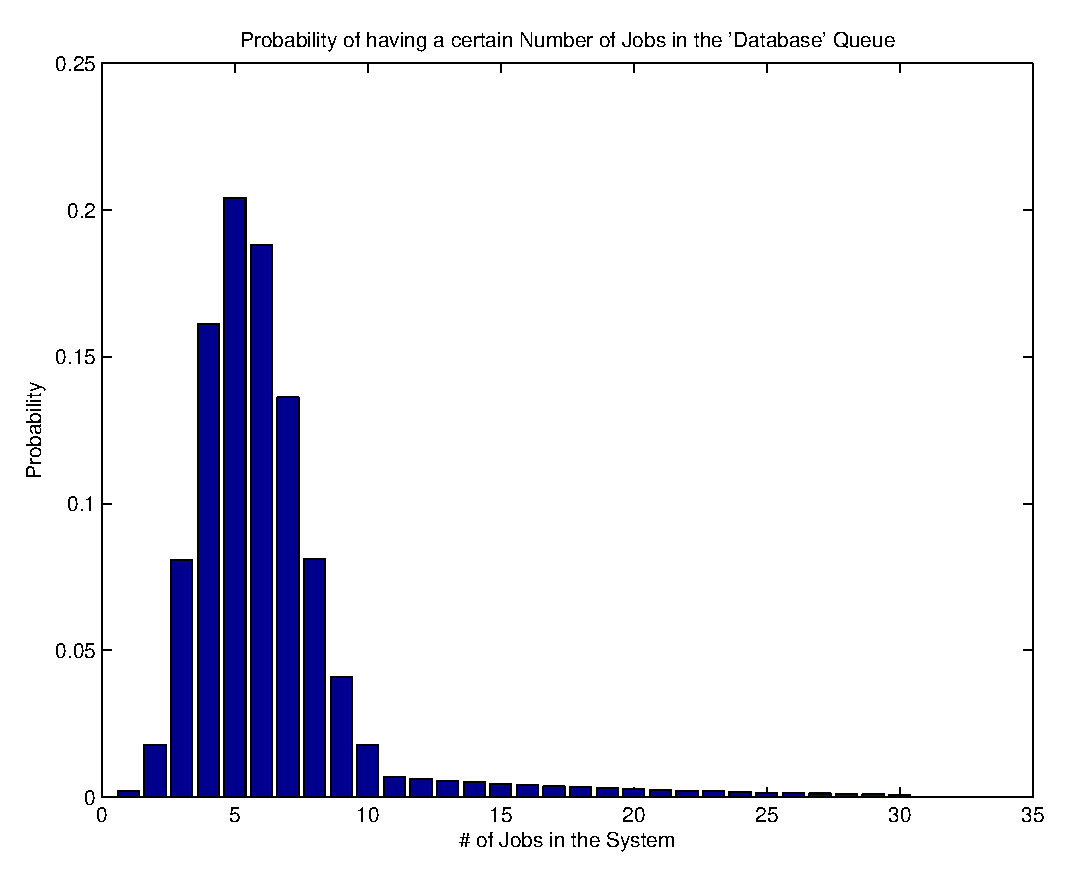
\includegraphics[scale=0.6]{../plots-ms2-mg/queueanalysis-3Db.eps}
  \end{center}
  \caption{Probability of having a certain Number of Jobs in the 'Database' Queue}
  \label{fig:queueanalysis3}
\end{figure}

%% ----------------------------------------------

\subsubsection{Explanation}
Having the database modelled like this results in a traffic intensity $\rho$ of $0.9$ which means that this service center is stable but under heavy load. The mean number of jobs in this is calculated to be $9$ which means that with $10$ processing nodes there is no queueing on average.


\subsection{Network Send - M/M/8}
Since this queue is symmetric to \ref{sub:QueueNwReceive} the characteristics is the same. One could consider to merge both queues 'Network Send' and 'Network Receive' together.

\subsection{Conclusion}

Having calculated some values for the modelled queues shows that one could switch off a few of the middleware instances while still being able to serve the same number of clients. All queues except for the database queue are on low load.

If the number of middleware instances would be halved to 4 the mean arrival rate per queue would be doubled. We would get the following numbers:


\nprounddigits{2}
\begin{figure}[H]
	\begin{center}
\begin{tabular}{|l|l|l|l|}
\hline 
& Network Receive & Process Request & Network Send \\
\hline

Traffic Intensity ($\rho$)
& \numprint{0.28125000000000000000000000000000000000000000000000}
& \numprint{0.09375000000000000000000000000000000000000000000000}
& \numprint{0.28125000000000000000000000000000000000000000000000}
\\

Probability of Queueing 
& \numprint{0.01180067807584736998300313857388238891336996501704}
& \numprint{0.00023489631212789959197640597042626430765036988919}
& \numprint{0.01180067807584736998300313857388238891336996501704}
\\

Mean \# of Jobs in the System 
& \numprint{1.1273854886344730523305484860203063032276050612876242968750000000000}
& \numprint{0.36830691758139397211463780018653707136797952272140}
& \numprint{1.1273854886344730523305484860203063032276050612876242968750000000}
\\

Mean \# of Jobs in the Queue 
& \numprint{0.0023854886344730523305484860203063032276050612876242968750000000}
& \numprint{0.00002429961849598961296307647969926872148107274708}
& \numprint{0.00238548863447305233054848602030630322760506128762429687500}
\\

\hline 
\end{tabular} 
	\end{center}
  	\caption{Calculated Queue Values with 4 middleware instances}
  	\label{fig:AnalyzeQueue4Broker}
\end{figure}

\npnoround



%% ----------------------------------------------
% Section Bottleneck Analysis
%% ----------------------------------------------
\section{Bottleneck Analysis}

A bottleneck analysis was performed to determine which component limits the total capacity of the system. Table \ref{tabular:BottleneckParams} shows the values required for this Analysis.

Row $S$ and $X$ are measurement values obtained from Milestone I. By applying \textit{Utilisation Law} (eq. \ref{eq:UtilisationLaw}) row $U$ can be calculated.   

\begin{equation}
\label{eq:UtilisationLaw}
U = X S
\end{equation}


The last row $D$ is obtained by combining \textit{Utilisation Law} and \textit{Forced Flow Law} (eq. \ref{eq:Demand}). 

\begin{equation}
\label{eq:Demand}
U = X_{total} D
\end{equation}


\begin{figure}[H]
\label{tabular:BottleneckParams}
\begin{center}
\begin{tabular}{|l|l|l|l|l|l|}
\hline 
 & \textbf{Network Receive} & \textbf{Process Request} & \textbf{Database} & \textbf{Network Send}\\ 
\hline
\textbf{$S$ Mean Service Time [ms]} & • & • & • & • \\
\hline 
\textbf{$X$ Throughput [req/min]} & • & • & • & • \\
\hline
\textbf{$U$ Utilisation} & • & • & • & • \\
\hline
\textbf{$D$ Demand} & • & • & • & • \\
\hline
\end{tabular} 
\caption{Bottleneck Analysis Input Parameters}
\end{center}
\end{figure}


- Mean Service Time per Device $S_i$\\
- Throughput per Device $X_i$


%% ----------------------------------------------
% Section MVA
%% ----------------------------------------------
\section{Mean-Value Analysis}

A Mean-Value Analysis was performed for the system. Because some of the queues are modelled to be load dependent the extended MVA algorithm from the book \cite[Box 36.1]{Raj} was implemented in java to perform this analysis.

\subsection{Model versus Measurement}
Plot \ref{fig:mva-rt} and \ref{fig:mva-tp} show the model estimated response time and throughput of the system. The red crosses show measured values.


% ------------------------------------------------
% Figure 

\begin{figure}[H]
	\begin{center}
    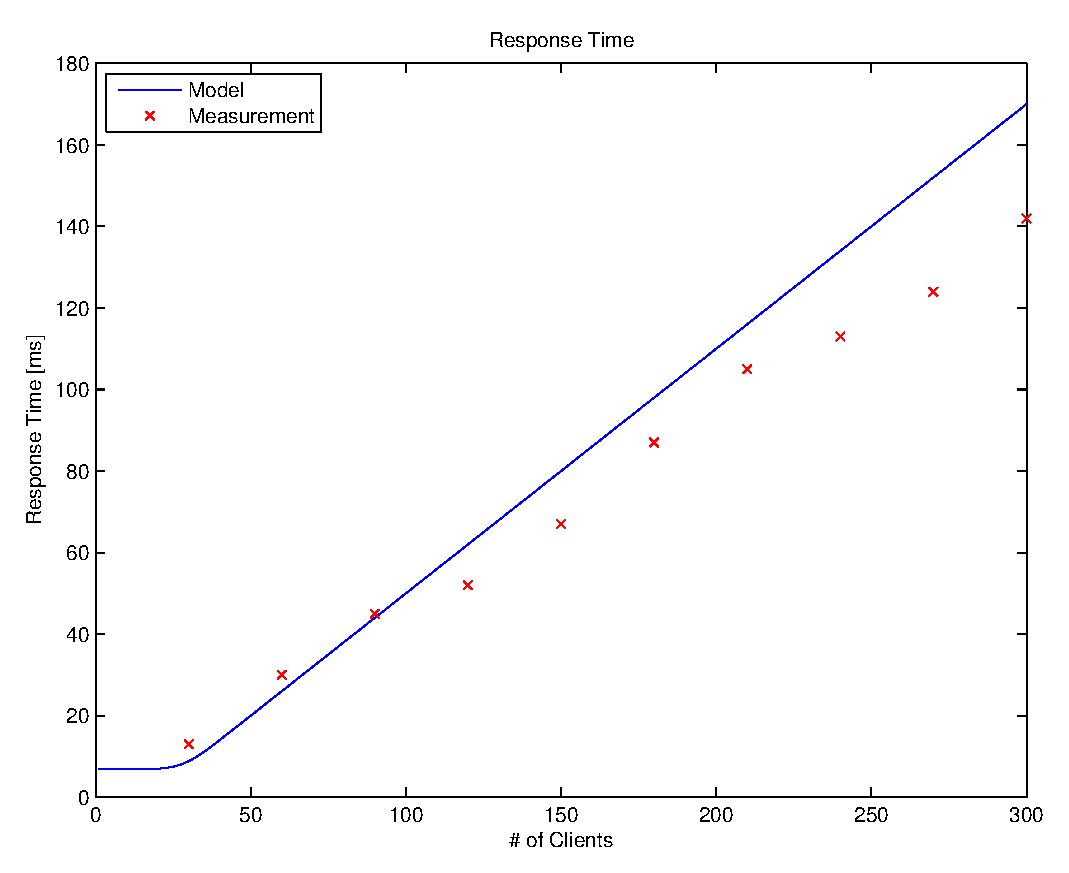
\includegraphics[scale=0.6]{../plots-ms2-mg/mva-rt.eps}
  \end{center}
  \caption{Mean Value Analysis Response Time}
  \label{fig:mva-rt}
\end{figure}

%% ----------------------------------------------

% ------------------------------------------------
% Figure 

\begin{figure}[H]
	\begin{center}
    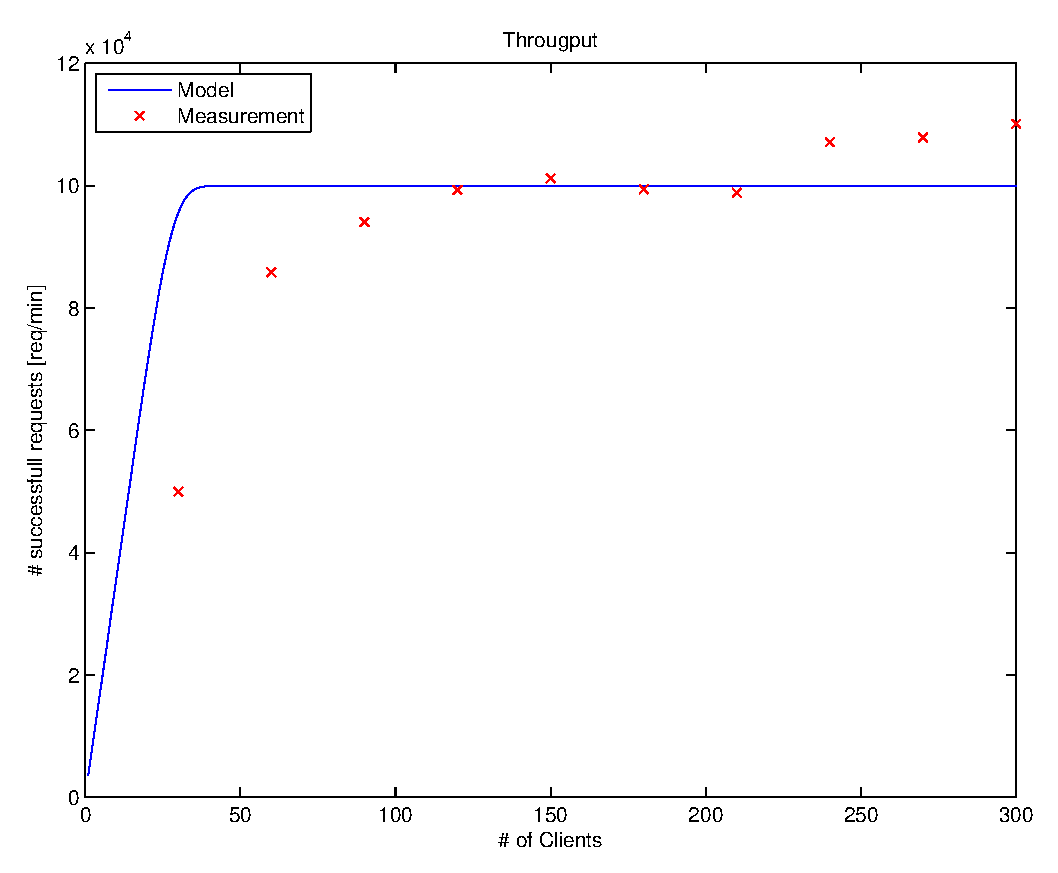
\includegraphics[scale=0.6]{../plots-ms2-mg/mva-tp.eps}
  \end{center}
  \caption{Mean Value Analysis Throughput}
  \label{fig:mva-tp}
\end{figure}

%% ----------------------------------------------


\subsubsection{Explanation}
Both graphs from the model match quite good with the measured values. However looking at the response time graph \ref{fig:mva-rt} the model graphs looks a bit steeper than the measured values (specially when looking at the $>200$ client values). Looking at the throughput graph \ref{fig:mva-tp} also shows a slight discrepancy in the same region. The measured values do not saturate at around $10'000$ requests per minute as the model graph does. A possible explanation may be variations while performing measurement at the Amazon cloud or marginally misstuned model parameters.


\subsection{Calculating Utilisation}

Figures 


% ------------------------------------------------
% Figure 

\begin{figure}[H]
	\begin{center}
    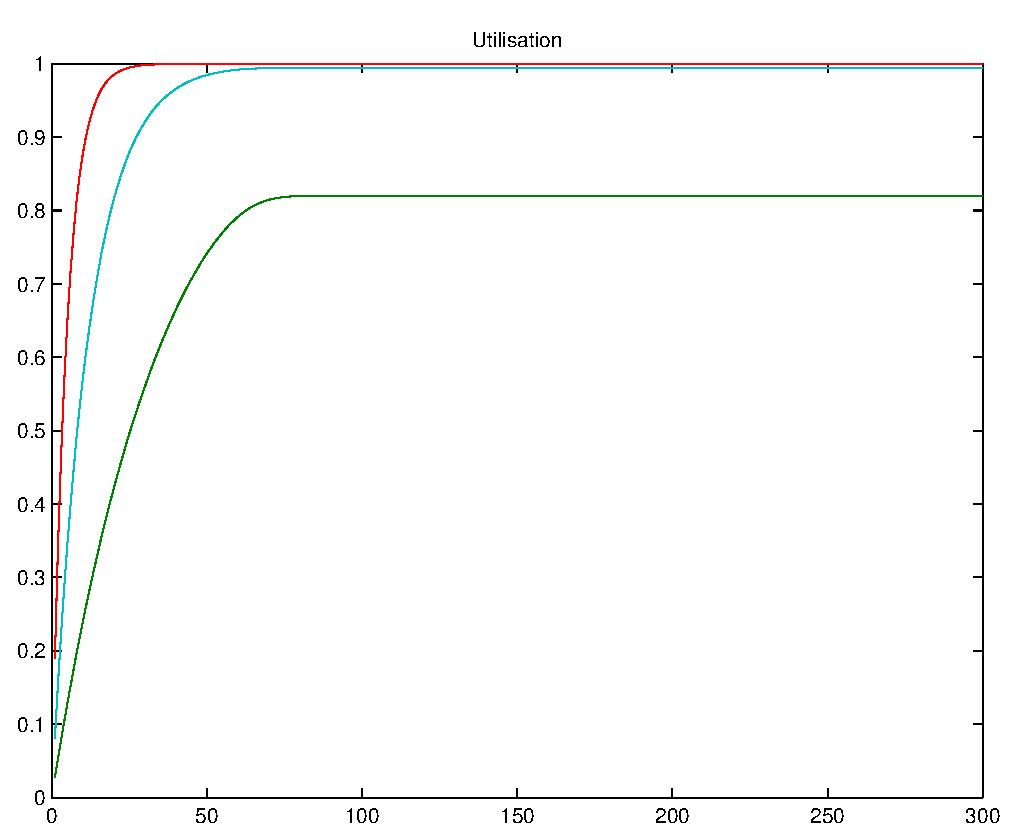
\includegraphics[scale=0.6]{../plots-ms2-mg/mva-utilisation.eps}
  \end{center}
  \caption{Mean Value Analysis Utilisation}
  \label{fig:mva-utilisation}
\end{figure}

%% ----------------------------------------------


% ------------------------------------------------
% Figure 

\begin{figure}[H]
	\begin{center}
    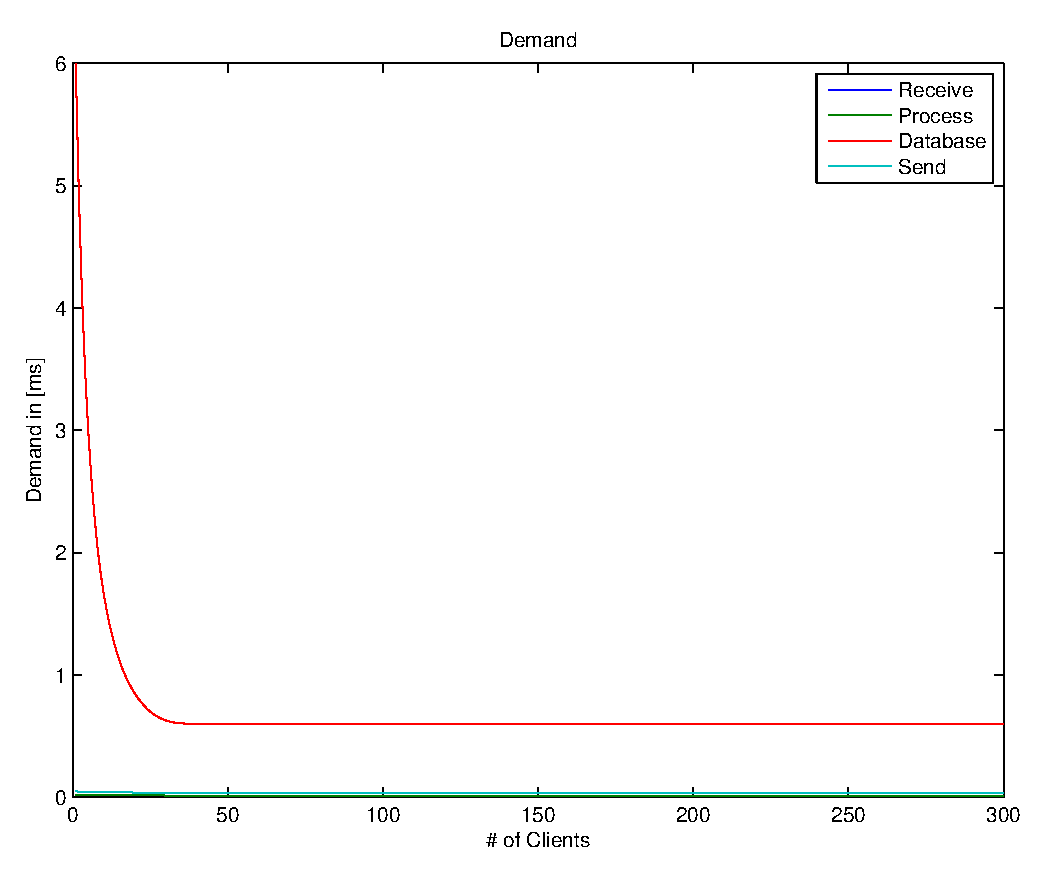
\includegraphics[scale=0.6]{../plots-ms2-mg/mva-demand.eps}
  \end{center}
  \caption{Mean Value Analysis Demand}
  \label{fig:mva-demand}
\end{figure}

%% ----------------------------------------------






% ------------------------------------------------
% Figure 

\begin{figure}[H]
	\begin{center}
    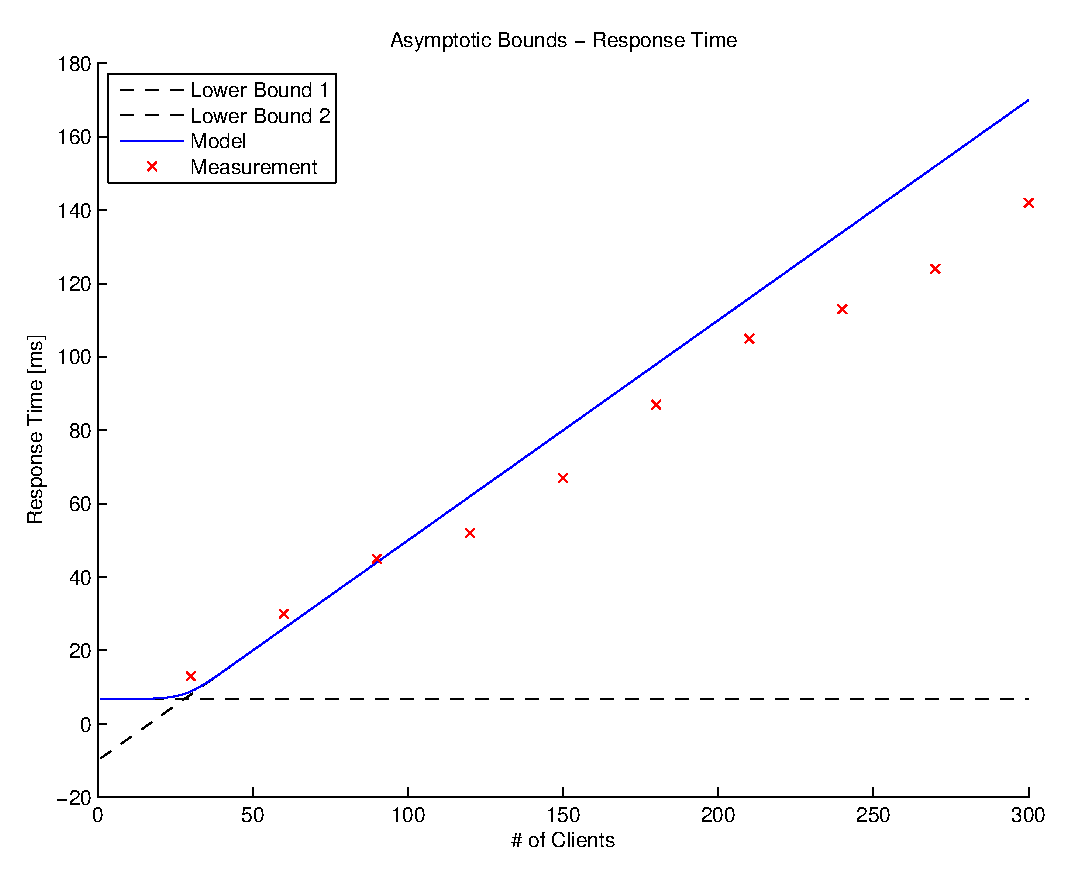
\includegraphics[scale=0.6]{../plots-ms2-mg/bottleneck-rt.eps}
  \end{center}
  \caption{Bottleneck Response Time}
  \label{fig:bottleneck-rt}
\end{figure}

%% ----------------------------------------------


% ------------------------------------------------
% Figure 

\begin{figure}[H]
	\begin{center}
    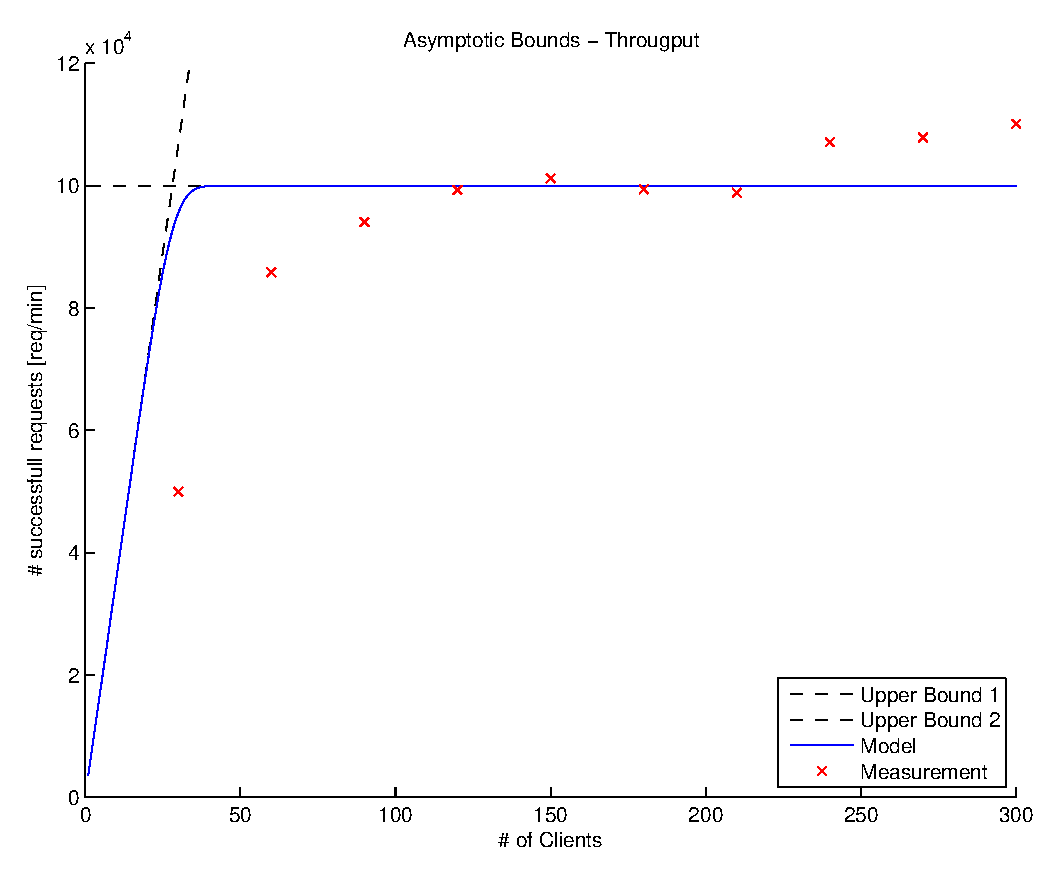
\includegraphics[scale=0.6]{../plots-ms2-mg/bottleneck-tp.eps}
  \end{center}
  \caption{Bottleneck Throughput}
  \label{fig:bottleneck-tp}
\end{figure}

%% ----------------------------------------------




%% ----------------------------------------------
% Section Experiments
%% ----------------------------------------------
\section{Experiment}
\label{sec:experiment}
For this milestone it was decided to repeat the experiment where the load is gradually increased until the system trashes. The previous one performed for milestone 1 was flawed because the number of clients were dynamically increased without stopping the measurements. Warmup time of the freshly connected clients were not considered properly.

\subsection{Experiment Setup}


\begin{figure}[H]
\label{tabular:experimentsetup}
\begin{center}
\begin{tabular}{|l|l|}
\hline 
\textbf{Parameter} & \textbf{Value} \\ 
\hline 
Broker & 8 distributed over 4 Amazon EC2 medium  instances (2 VCU per instance)\\ 
\hline 
\# of Worker Thread & 20 per middleware \\
\hline 
\# of DB Connections & 15 per middleware \\
\hline 
Client Type & OneWayClient \\ 
\hline 
Client Think Time & 10ms \\ 
\hline 
\# of Clients & 30 - 300 \\ 
\hline 
Request Timeout & 1 s\\
\hline 
Experiment Duration & 7min \\ 
\hline 
\end{tabular} 
%\caption{Experiment Parameters}
\end{center}
\end{figure}


\subsection{Hypothesis}

By increasing the load on the system both response time and throughput should increase to
a certain degree. By increasing the load more the system should become unstable and start
trashing.

\subsection{Result}


% ------------------------------------------------
% Figure 

\begin{figure}[H]
	\begin{center}
    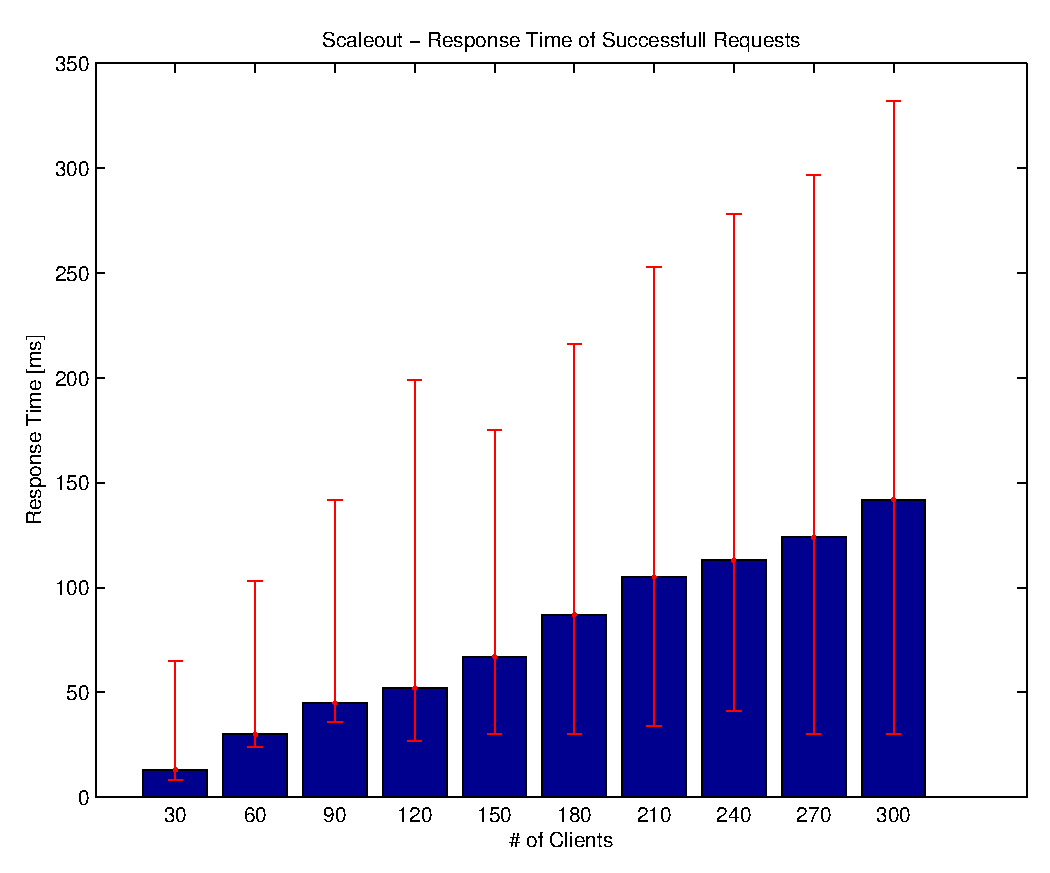
\includegraphics[scale=0.6]{../plots-ms2-mg/experiment-rt.eps}
  \end{center}
  \caption{Histogram showing Response Times\newline(Error bars are the 2.5\% and 97.5\% percentiles)}
  \label{fig:experiment-rt}
\end{figure}

%% ----------------------------------------------


% ------------------------------------------------
% Figure 

\begin{figure}[H]
	\begin{center}
    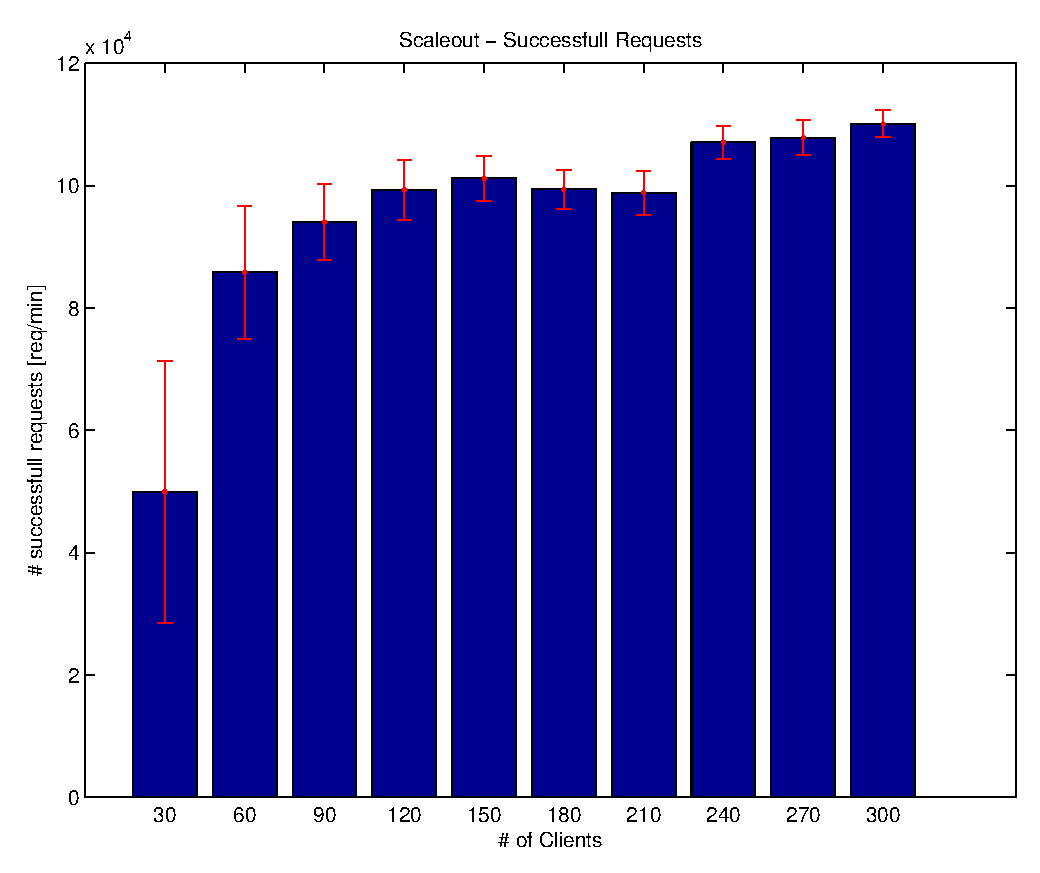
\includegraphics[scale=0.6]{../plots-ms2-mg/experiment-tp.eps}
  \end{center}
  \caption{Histogram showing number of successfull Requests\newline(Error bars are standard deviation)}
  \label{fig:experiment-tp}
\end{figure}

%% ----------------------------------------------

% ------------------------------------------------
% Figure 

\begin{figure}[H]
	\begin{center}
    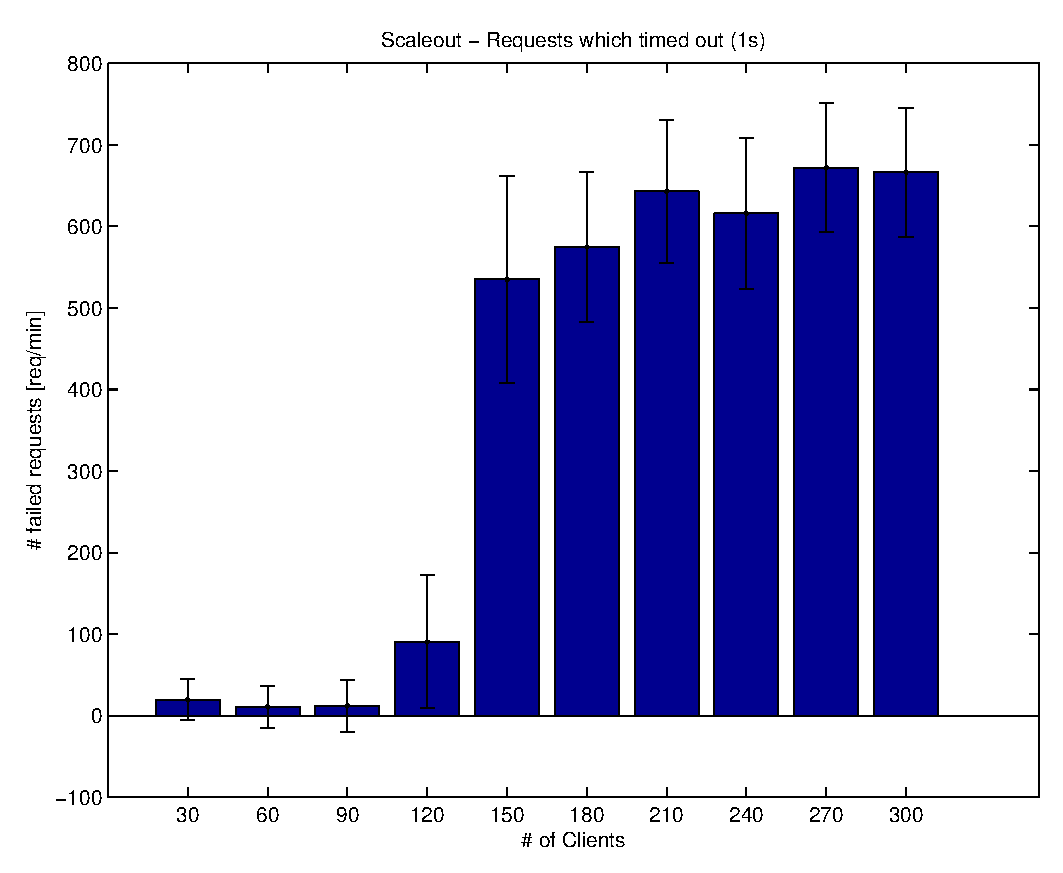
\includegraphics[scale=0.6]{../plots-ms2-mg/experiment-err.eps}
  \end{center}
  \caption{Histogram showing Failed Requests\newline(Error bars are standard deviation)}
  \label{fig:experiment-error}
\end{figure}

%% ----------------------------------------------

\subsection{Sanity Check}

The measured data can be check if they are plausible using the \textit{Interactive Response Time Law}.

\begin{equation}
\label{eq:InteractiveResponseTimeLaw}
X = {{N} \over {R + Z}}
\end{equation}


Where $X$ is the throughput, $N$ the number of clients, $R$ the response time and $Z$ the think 	time. Table \ref{tabular:experimentsanitycheck} shows the table containing the measured values. Column $Z$ was calculated based on the measured values $X$ and $R$ using formula \ref{eq:InteractiveResponseTimeLaw}. 

\begin{figure}[H]
\label{tabular:experimentsanitycheck}
\begin{center}
\begin{tabular}{|r|r|r|r|}
\hline 
$N$ & $X$ [req/min] & $R$ [ms] & $Z$ [ms]\\
\hline 
30&	49970&	20&	16\\
60&	85833&	32&	10\\
90&	94047&	48&	9\\
120&	99332&	60&	12\\
150&	101191&	72&	17\\
180&	99415&	92&	17\\
210&	98858&	109&	18\\
240&	107105&	116&	18\\
270&	107871&	130&	20\\
300&	110108&	147&	16\\
\hline 
\end{tabular} 
\caption{Calculated Think Time}
\end{center}
\end{figure}


\subsection{Interpretation}

As expected while adding more and more clients the response time and its variance gradually increases. As seen in figure \ref{fig:experiment-tp} The system seems to saturate at about 100'000 requests per minute. This load is reached between 90 and 100 clients. From this point on both variance of response time and number of requests which can not be processed within the 1 second timeout time drastically increase. This can be seen in figure \ref{fig:experiment-error} where the number of requests which have not been processed jumps while scaling the number of clients.

A flaw in the experiment can be observed in figure \ref{fig:experiment-rt}. The 30 client bar has a very high variance. This is because 30 client produce less load (thuss less measurement values) than 300. To fix this issue the 30 client experiment should have been run for a longer period of time. This should have reduced measurement variance.

Another observation is that more data points between 0 and 100 clients should have been taken to get more confidence about what's happening when the system is not yet saturated.

The calculated think time $Z$ has the expected magnitude and does not vary too much (around 15ms). The measured data seem to be plausible.


\pagebreak


\bibliographystyle{plain}
\bibliography{literature}


\end{document}

